\documentclass{beamer}
\usepackage[utf8]{inputenc}
\usetheme{Warsaw}
\title[Slovenski NLTK označevalnik]{Slovenski NLTK označevalnik}
\author{
	Niko Colnerič
	\and
	Nejc Banič}
\institute{ Fakulteta za Računalništvo in Informtiko\\
			Univerza v Ljubljani}

\begin{document}

\begin{frame}
\titlepage
\end{frame}

\begin{frame}{Motivacija}
This is a short introduction to Beamer class.
\end{frame}

\begin{frame}{Implementirani označevalniki}
\begin{itemize}
\item \textbf{Trigram označevalnik}\\
\textit{a priori najbolj verjetno oznako v kontekstu dolžine 3}
\begin{center}
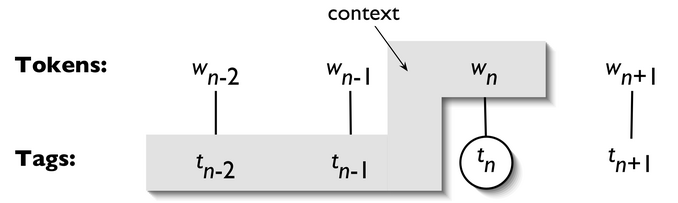
\includegraphics[width=0.6\textwidth]{../paper/tag-context.png}
\end{center}

\item \textbf{Brillov označevalnik}\\
\textit{ugane oznako vsako besede, nato 
popravi svoje napake tako, da uporabi seznam transformacijskih pravil}
\item označevalnik na podlagi \textbf{naivnega Bayes-ovega klasifikatorja}\\
\textit{predpostavi pogojno neodvisnost atributov pri danem razredu}
\end{itemize}
\end{frame}

\begin{frame}{JOS korpus}

Osnovna komponenta za izgradnjo slovenskega NLTK označevalnik je JOS korpus. Vsebuje zbirko različnih besedil s podrobno ročno preverjenimi jezikoslovnimi oznakami (npr. leme, oblikoskladenjske oznake itd.). Korpus je kompatibilen z MULTEXT-East V4 oblikoskladenjskimi specifikacijami (ang. \textit{morphosyntactic descriptions (MSDs)}), ki definirajo kategorije (besedne vrste) za slovenski jezik, za vsako kategorijo pa tudi njene atribute in njihove vrednosti. Uporabila sva korpus \textit{jos1M}, ki vsebuje 1 milijon besed z delno ročno preverjenimi lemami in oblikoskladenjskimi oznakami. Struktura JOS korpusa je zapisana v XML.
\end{frame}

\begin{frame}{NLTK trainer}
\end{frame}

\begin{frame}{Postopek treniranja označevalnikov}
\begin{enumerate}
\item Transformacija \textit{.XML} korpusa v \textit{.pos}
\item Treniranje z skripto iz NLTK-trainer
\item Ocenjevanje točnosti
\item Ocenjevanje hitrosti
\end{enumerate}
\end{frame}

\begin{frame}{Primer}
\begin{center}
\textit{\textbf{Lep je dan, vse diši že po pomladi}}
\end{center}
\textit{( Lep  |  PPNMEIN ) - pridevnik\\
	( je  |  GP-STE-N ) - glagol\\
	( dan  |  SOMEI ) - samostalnik\\
	( ,  |  , ) - ni razlage\\
	( vse  |  ZC-SEI ) - zaimek\\
	( diši  |  GGNSTE ) - glagol\\
	( že  |  L ) - členek\\
	( po  |  DM ) - predlog\\
	( pomladi  |  SOZEM ) - samostalnik\\
	( !  |  ! ) - ni razlage}\\
\end{frame}

\begin{frame}{Celoten MSD za \textit{Lep} }
\begin{center}
\begin{tabular}{c|c}
\multicolumn{2}{c}{pridevnik}\\\hline\hline
vrsta & splošni \\
spol & moški \\
število & ednina \\
sklon & imenovalnik \\
živost & 0 \\
vid & 0 \\
oblika & 0 \\
oseba & 0 \\
nikalnost & 0 \\
stopnja & nedoločeno \\
določnost & ne \\
število\_svojine & 0 \\
spol\_svojine & 0 \\
naslonskost & 0 \\
zapis & 0 \\
\end{tabular}
\end{center}
\end{frame}

\begin{frame}{Rezultati natančnost}
\begin{figure}[h]
\begin{center}
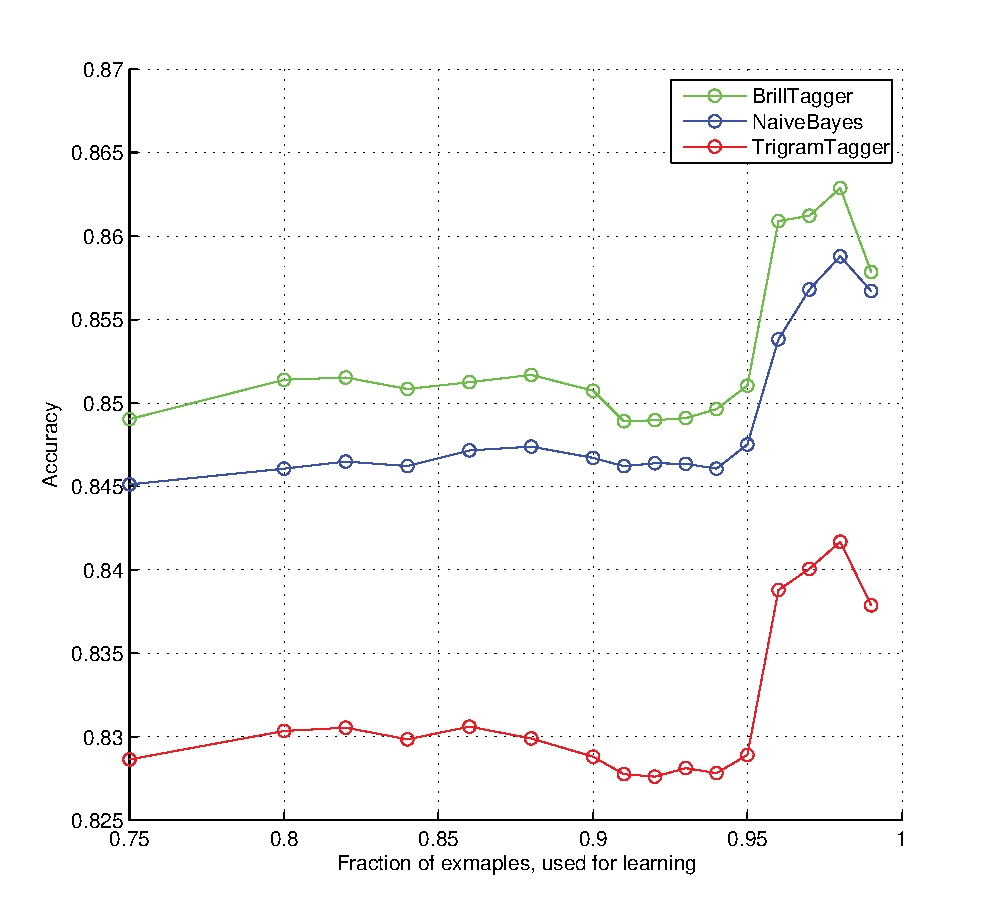
\includegraphics[height=0.85\textheight]{../evaluation/graph.pdf} 
\end{center}
\end{figure}
\end{frame}

\begin{frame}{Rezultati hitrost}
\begin{figure}[h]
\begin{center}
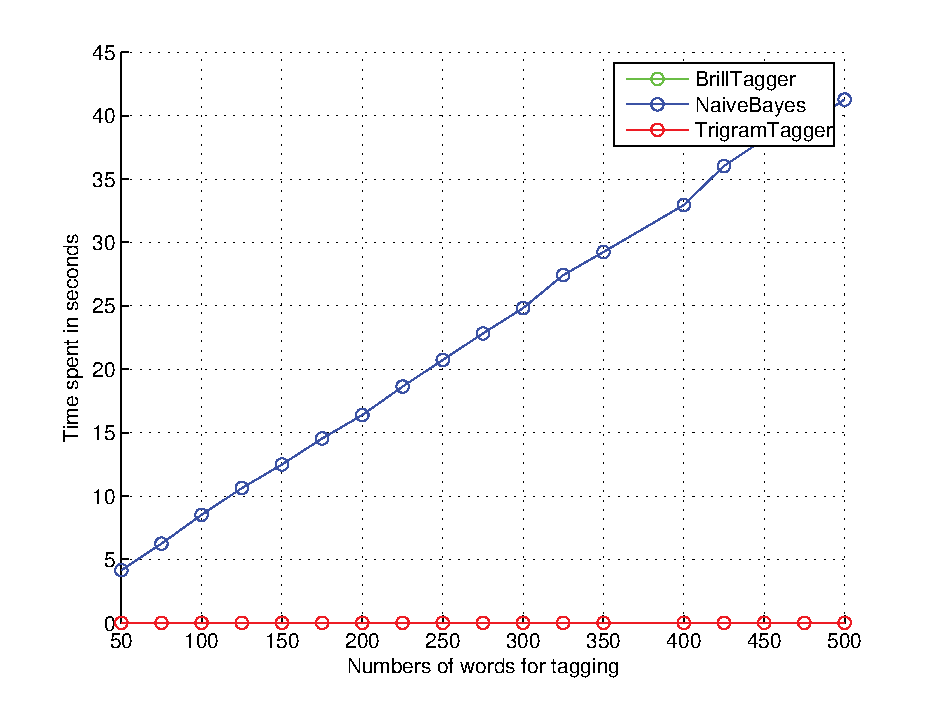
\includegraphics[height=0.85\textheight]{../evaluation/graph_speed.pdf} 
\end{center}
\end{figure}
\end{frame}

\begin{frame}{Zaključek, izboljšave}

Ne moreva trditi, da so uporabljeni označevalniki (Trigram, Brill in naivni Bayes) najhitrejši in najbolj natančni. Zato je ena možnost za izboljšavo uporaba drugih označevalnikov. 
\par
Če bi hotela izboljšati natančnost naših označevalnik, bi lahko v proces učenja uporabila tudi drugih korpuse. 

\par
Označevanje v slovenskem jeziku je praktično z uporabo knjižnice \textit{Natural Language Toolkit} in projekta nltk-trainer. Evalvacija je pokazala, da sta tako Brill kot Trigram označila besede hitro, medtem ko je bil naivni Bayes-ov klasifikator veliko počasnejši. Razlike v natančnosti vseh treh označevalnikov praktično ni.
\end{frame}
\end{document}